\documentclass[a4paper,10pt]{report}

\usepackage{packages/rapportutc}
%\usepackage{packages/include-packages}


%%%%%%%% Références %%%%%%%%
\usepackage{cleveref}
\usepackage{hyperref}
\usepackage[nottoc, notlof, notlot]{tocbibind} % bibliographie http://tex.stackexchange.com/questions/71129/bibliography-in-table-of-contents
\usepackage{natbib} % bibliographie

%%%%%%%% Code informatique %%%%%%%%
\usepackage{packages/Sweave} %package d'affichage des codes R
\usepackage{listings} % pour hightlight code

%%%%%%%% Formules mathématiques %%%%%%%%
\usepackage{amsmath, amsthm, amssymb, graphics, setspace} %packages de mathématiques
\usepackage{chemist} %formule chimique 

%%%%%%%% Mise en forme %%%%%%%%
% Mise en forme graphique
\usepackage{graphicx,wrapfig,lipsum} % pour afficher des figures à côté du texte
\usepackage[linewidth=1pt]{mdframed} % permet de générer et gérer des frames
\usepackage{rotating} % rotations on tables, captions, text, ...
% Mise en forme images et tableaux
\usepackage{float} % permet de spécifier l'option "H" aux captions afin de les positionner de manière fixe
\usepackage{subcaption} % permet d'afficher plusieurs images dans une caption
\usepackage{array} % meilleurs "table" et "tabular"
% Mise en forme texte
\usepackage{setspace} % permet de spécifier l'espacement interligne
\usepackage{ulem} % \sout{Texte à barrer} \xout{Texte à hachurer} \uwave{Texte à souligner par une vaguelette}
\usepackage{calc,enumitem}  % Mise en forme l'environnement itemsize description etc.
\usepackage{color} % utilisation de couleurs
\usepackage{ae,aecompl} % Vir­tual fonts for T1 en­coded CMR-fonts
\usepackage{pifont} % com­mands for Pi fonts (Ding­bats, Sym­bol, etc.)
\usepackage{comment} % Selectively include/exclude portions of text \comment....\endcomment

\onehalfspacing % espacement interligne
\setlength{\parindent}{.5em} % indentation des retraits de première ligne

%%%%%%%%%%%%%%%%%%%%%%%%%%%%%%%%%%%%%%%%%%%%%%%%%%%%%%%%%%%%%%%%%%%%%%%%%%%% 

\title{TP 2 - Classification automatique}
\author{LU Han - HAMONNAIS Raphaël}
\date{\today}

\uv{SY09}
\branche{Génie Informatique}
\filiere{Fouille de Données et Décisionnel}
%%%%%%%%%%%%%%%%%%%%%%%%%%%%%%%%%%%%%%%%%%%%%%%%%%%%%%%%%%%%%%%%%%%%%%%%%%%%

\begin{document}

\renewcommand{\labelitemi}{\large\textcolor{tatoebagreen}{\fg}}
\newgeometry{top=2.5cm,bottom=2cm,left=2cm,right=2cm}
\groovypdtitre
\restoregeometry % restaure la géométrie par défaut de latex

%%%%%%%%%%%%%%%%%%%%%%%%%%%%%%%%%%%%%%%%%%%%%%%%%%%%%%%%%%%%%%%%%%%%%%%%%%%% 

\tableofcontents

%%%%%%%%%%%%%%%%%%%%%%%%%%%%%%%%%%%%%%%%%%%%%%%%%%%%%%%%%%%%%%%%%%%%%%%%%%%%



\chapter{Visualisation des données}

\section{Visualisation des données Iris}

\begin{figure}[H]
	\centering
	\captionsetup{justification=centering, margin=2cm}
	\caption{\small Représentation des données \texttt{Iris} dans le premier plan factoriel après ACP}
	\begin{subfigure}[b]{0.5\linewidth}
		\centering
		\captionsetup{justification=centering, margin=1cm}
		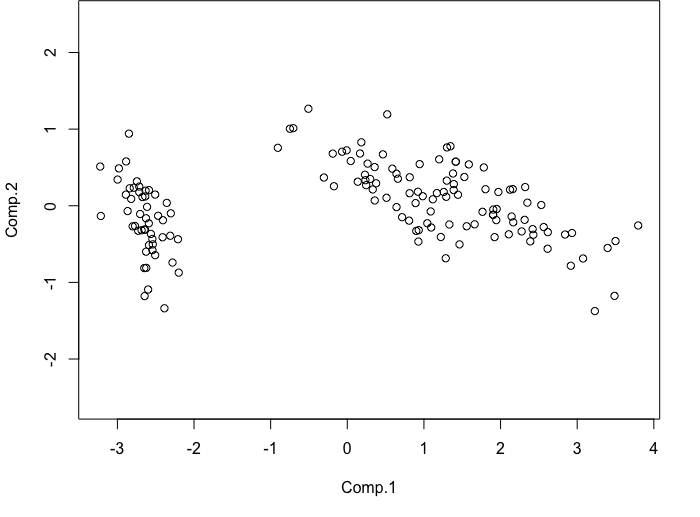
\includegraphics[width=1\linewidth]{img/1-iris-acp-premier-plan-factoriel}
		\caption{\scriptsize Données \texttt{Iris} dans le premier plan factoriel sans tenir compte de l'espèce}
		\label{fig:1-iris-acp-premier-plan-factoriel}
	\end{subfigure}%
	\begin{subfigure}[b]{0.5\linewidth}
		\centering
		\captionsetup{justification=centering, margin=1cm}
		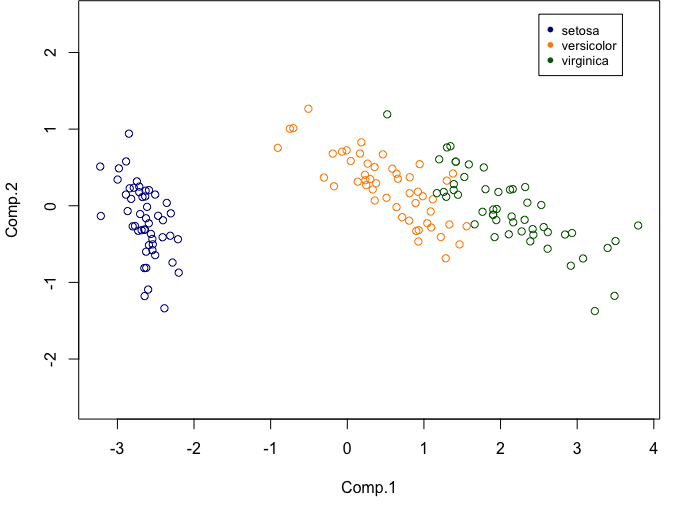
\includegraphics[width=1\linewidth]{img/1-iris-acp-premier-plan-factoriel-discr-species}
		\caption{\scriptsize Données \texttt{Iris} dans le premier plan factoriel en tenant compte de l'espèce}
		\label{fig:1-iris-acp-premier-plan-factoriel-discr-species}
	\end{subfigure}%
	
	\label{fig:1-iris-acp-representation-graphique}%
\end{figure}

\begin{itemize}
	\item Affichage dans le premier plan factoriel sans tenir compte de l'espèce
	\begin{itemize}
		\item On observe deux groupes bien distincts (voir \autoref{fig:1-iris-acp-premier-plan-factoriel}).
	\end{itemize}

	\item Affichage dans le premier plan factoriel en tenant compte de l'espèce
	\begin{itemize}
		\item On voit qu'un des deux groupes précédemment observé est en fait constitué de deux espèces différentes (voir \autoref{fig:1-iris-acp-premier-plan-factoriel-discr-species})~;
		\item On obtient donc deux informations précieuses~:
		\begin{itemize}
			\item Les méthodes de classification géométriques tendront à nous donner deux classes ;
			\item On sait que les données contiennent en réalité trois classes bien distinctes quand le facteur discriminant est l'espèce ;
			\item Il faudra donc faire attention à ce qu'on cherche à obtenir~: une nouvelle classification en X classes sans tenir compte de l'espèce, et auquel cas on obtiendra surement deux classes. Ou bien une classification en fonction de l'espèce et alors il faudra spécifier qu'on cherche à obtenir trois classes.
		\end{itemize}
	\end{itemize}
\end{itemize}





\section{Visualisation des données Crabs}

\begin{figure}[H]
	\centering
	\captionsetup{justification=centering, margin=2cm}
	\caption{\small Représentation des données \texttt{Crabs} dans le premier plan factoriel après ACP}
	\begin{subfigure}[b]{0.5\linewidth}
		\centering
		\captionsetup{justification=centering, margin=1cm}
		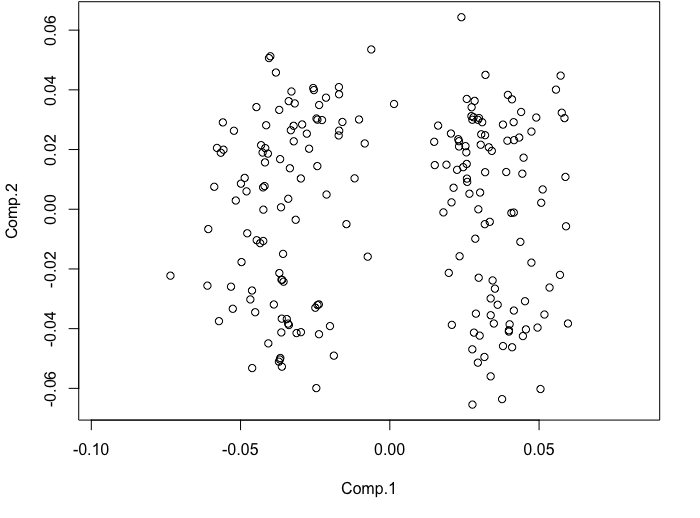
\includegraphics[width=1\linewidth]{img/1-crabs-acp-premier-plan-factoriel}
		\caption{\scriptsize Données \texttt{Crabs} dans le premier plan factoriel sans tenir compte de l'espèce ou du sexe}
		\label{fig:1-crabs-acp-premier-plan-factoriel}
	\end{subfigure}%
	\begin{subfigure}[b]{0.5\linewidth}
		\centering
		\captionsetup{justification=centering, margin=1cm}
		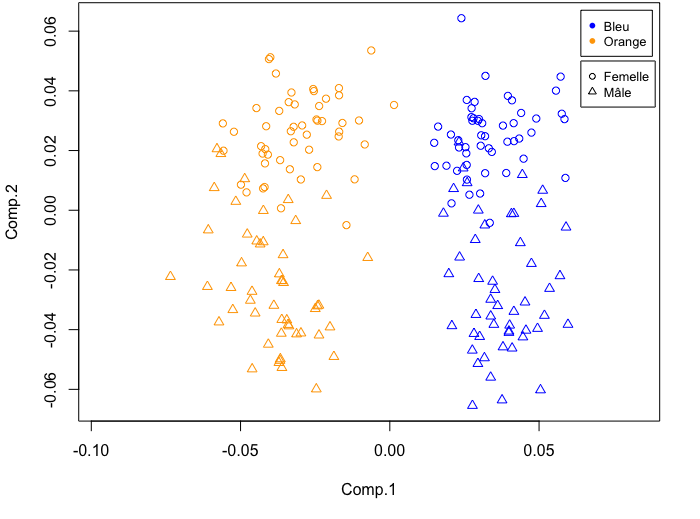
\includegraphics[width=1\linewidth]{img/1-crabs-acp-premier-plan-factoriel-discr-species-and-sex}
		\caption{\scriptsize Données \texttt{Crabs} dans le premier plan factoriel en tenant compte de l'espèce et du sexe}
		\label{fig:1-crabs-acp-premier-plan-factoriel-discr-species-and-sex}
	\end{subfigure}%
	\label{fig:1-crabs-acp-representation-graphique}%
\end{figure}


\begin{itemize}
	\item Affichage dans le premier plan factoriel sans tenir compte de l'espèce ou du sexe
	\begin{itemize}
		\item On observe deux groupes bien distincts (voir \autoref{fig:1-crabs-acp-premier-plan-factoriel}).
	\end{itemize}
	
	\item Affichage dans le premier plan factoriel en tenant compte de l'espèce et du sexe (voir \autoref{fig:1-crabs-acp-premier-plan-factoriel-discr-species-and-sex})
	\begin{itemize}
		\item On constate que les deux groupes observés précédemment correspondent à l'espèce des crabes ;
		\item On voit aussi apparaître deux autres groupes au sein des premiers qui délimitent le sexe ;
		\item On va donc chercher à faire une classification à 4 classes ;
		\item On note quand même que la délimitation entre les sexes est plus floue que celle entre les espèces.
	\end{itemize}
\end{itemize}



\section{Visualisation des données Mutation}

Les données \texttt{Mutation} représentent par le biais d'une matrice de dissimilarités les liens entre espèces~: plus la distance (dissimilarité) est faible, plus les espèces sont proches.

Nous allons effectuer une Analyse Factorielle de Tableau de Distance (AFTD). On rappelle que l’AFTD peut être vue comme un équivalent de l’ACP pour des données se présentant sous la forme d’un tableau $n \times n$ de dissimilarités $\delta_{ij}$ entre $n$ individus ($i,\ j \in \{1,...,n\}$)~: elle calcule une représentation multidimensionnelle de ces individus (dont le tableau de dissimilarités ne donne qu’une description implicite) dans un espace euclidien de dimension $p \leqslant n$. Cette représentation est exacte lorsque les dissimilarités sont des distances euclidiennes, ce qui n'est pas toujours le cas.
\\Après sélection d’un certain nombre de variables, la qualité de la représentation peut être évaluée numériquement par un critère similaire au pourcentage d’inertie de l’ACP, ou graphiquement au moyen d’un diagramme de Shepard : sur ce graphique, la distance $d_{ij} = d(x_i,x_j)$ entre les représentations de $x_i$ et $x_j$ déterminées par l’AFTD est représentée en fonction de la dissimilarité initiale $\delta_{ij}$, pour chaque couple d’individus $(x_i,x_j)$.


\subsection{Données Mutation dans le premier plan factoriel après AFTD}
\label{subsection:1-3-1-mut-premier-plan-factoriel}

\begin{figure}[H]
	\centering
	\captionsetup{justification=centering, margin=4cm}
	\caption{\small Représentation euclidienne des données \texttt{Mutation} en deux dimensions par AFTD}
	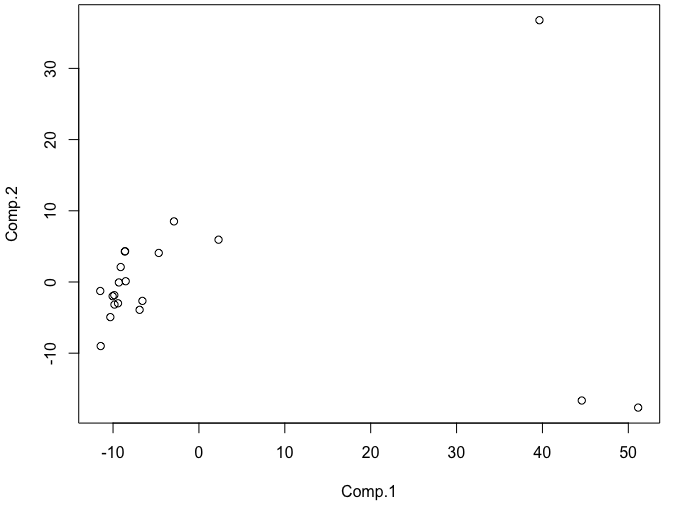
\includegraphics[width=.5\linewidth]{img/1-mut-acp-aftd-premier-plan-factoriel}
	\label{fig:1-mut-acp-aftd-deux-dimensions}%
\end{figure}


Cette représentation a le mérite de nous permettre d'appréhender plus facilement le tableau de dissimilarités~: on voit clairement que beaucoup des espèces sont proches les unes des autres. Certaines très proches. On voit aussi que trois d'entre elles sont particulièrement éloignées.

On pourrait former deux classes~: la première regroupant l'ensemble des points proches, et la seconde les trois points éloignés. Ou bien trois, si on décide que l'espèce tout en haut à droite du graphique est trop loin pour être intégrée à une classe. Il est aussi tout à fait possible de subdiviser la première classe d'espèces proches les unes des autres en plusieurs classes plus petites.




\subsection{Analyse de la qualité de la représentation par AFTD}

Certaines des valeurs propres (inertie expliquée de la composante principale correspondante) sont négatives. Calculer le pourcentage d'inertie expliquée demande alors de faire un choix~: transformer les valeurs propres négatives en leur inverse positif (valeur absolue) ou bien ne tenir compte que des valeurs propres positives. Nous avons ici effectué les calculs avec les deux possibilité afin de comparer les résultats (voir \autoref{table:1-mut-acp-aftd-inertie-valeurs-absolues} et \autoref{table:1-mut-acp-aftd-inertie-valeurs-positives}).

\begin{table}[H]
	\centering
	\caption{Inertie avec valeurs absolues}
	\begin{tabular}{r|rrrrr}
		& Comp.1 & Comp.2 & Comp.3 & Comp.4 & Comp.5 \\ 
		\hline
		\small Pourcentage d'inertie expliquée & 52.71 & 16.01 & 10.94 & 6.72 & 4.78 \\ 
		\small Pourcentage cumulé d'inertie expliquée & 52.71 & 68.72 & 79.67 & 86.38 & 91.16 \\ 
	\end{tabular}
	\label{table:1-mut-acp-aftd-inertie-valeurs-absolues}
\end{table}

\begin{table}[H]
	\centering
	\caption{Inertie avec valeurs positives seulement}
	\begin{tabular}{r|rrrrr}
		& Comp.1 & Comp.2 & Comp.3 & Comp.4 & Comp.5 \\ 
		\hline
		\small Pourcentage d'inertie expliquée & 53.43 & 16.23 & 11.09 & 6.81 & 4.84 \\ 
		\small Pourcentage cumulé d'inertie expliquée & 53.43 & 69.66 & 80.75 & 87.56 & 92.40 \\ 
	\end{tabular}
	\label{table:1-mut-acp-aftd-inertie-valeurs-positives}
\end{table}

On remarque que les pourcentages d'inertie expliquée ne varient pas énormément entre les deux choix de calcul. Cela s'explique par la faible importance des valeurs propres négatives dans ce jeu de données.

Pour ce qui est de la qualité de la représentation, on voit très vite qu'avec simplement deux dimensions, on n'obtient qu'environ 69\% d'inertie expliquée. C'est relativement peu pour une ACP, mais cela peut être suffisant pour une représentation simple des données. Tenir compte de trois, quatre ou cinq dimensions nous permet à chaque fois de mieux représenter des données, avec respectivement 80\%, 87\% et 92\% d'inertie cumulée.\\

On remarque aussi cette augmentation de qualité de représentation des données initiales lorsqu'on regarde les diagrammes de Shepard~:

\begin{figure}[H]
	\centering
	\captionsetup{justification=centering, margin=3cm}
	\caption{\small Diagrammes de Shepard pour les dimensions 2 à 5}
	\begin{subfigure}[b]{0.25\linewidth}
		\centering
		\captionsetup{justification=centering}
		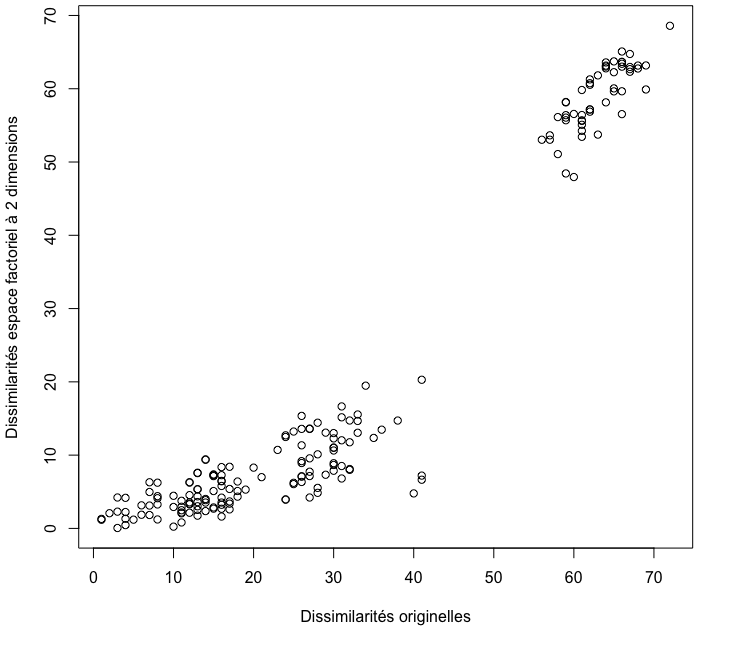
\includegraphics[width=1\linewidth]{img/1-mut-acp-aftd-diag-shepard-2-dim}
		\caption{\scriptsize Diagramme de Shepard\\(2 dimensions)}
		\label{fig:1-mut-acp-aftd-diag-shepard-2-dim}
	\end{subfigure}%
	\begin{subfigure}[b]{0.25\linewidth}
		\centering
		\captionsetup{justification=centering}
		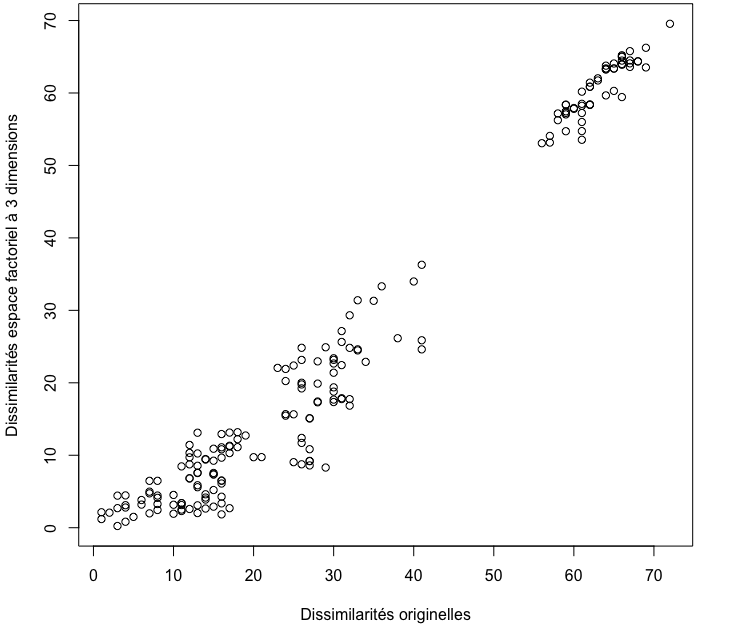
\includegraphics[width=1\linewidth]{img/1-mut-acp-aftd-diag-shepard-3-dim}
		\caption{\scriptsize Diagramme de Shepard\\(3 dimensions)}
		\label{fig:1-mut-acp-aftd-diag-shepard-3-dim}
	\end{subfigure}%
	\begin{subfigure}[b]{0.25\linewidth}
		\centering
		\captionsetup{justification=centering}
		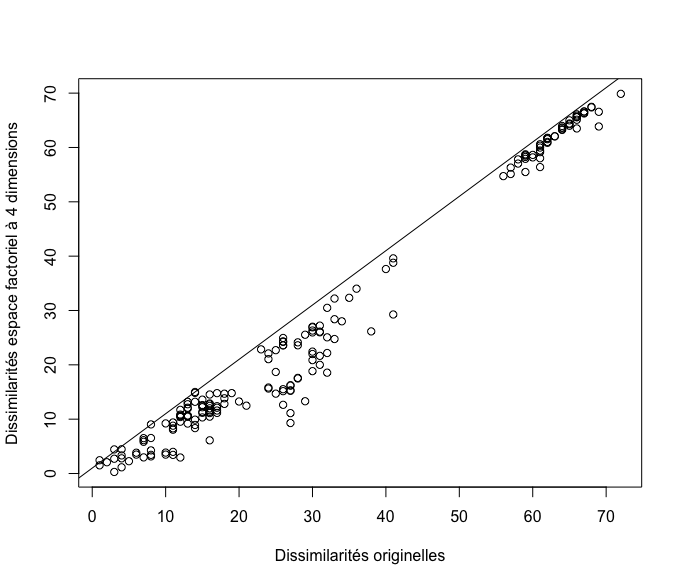
\includegraphics[width=1\linewidth]{img/1-mut-acp-aftd-diag-shepard-4-dim}
		\caption{\scriptsize Diagramme de Shepard\\(4 dimensions)}
		\label{fig:1-mut-acp-aftd-diag-shepard-4-dim}
	\end{subfigure}%
	\begin{subfigure}[b]{0.25\linewidth}
		\centering
		\captionsetup{justification=centering}
		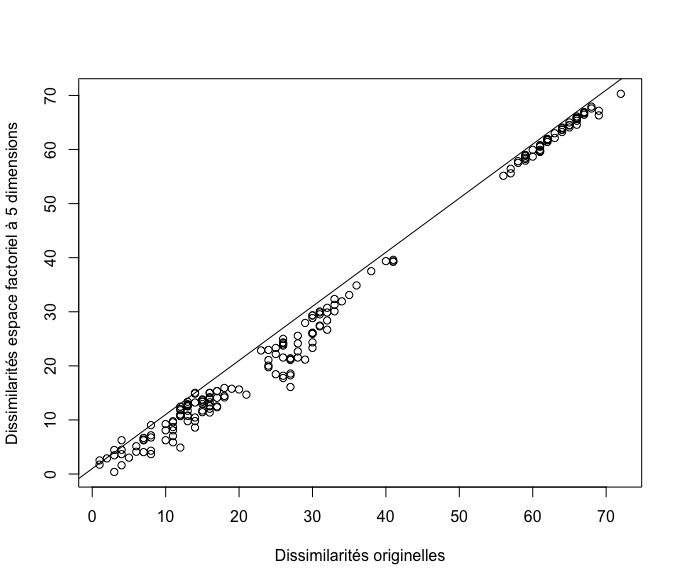
\includegraphics[width=1\linewidth]{img/1-mut-acp-aftd-diag-shepard-5-dim}
		\caption{\scriptsize Diagramme de Shepard\\(5 dimensions)}
		\label{fig:1-mut-acp-aftd-diag-shepard-5-dim}
	\end{subfigure}%
	\label{fig:1-mut-acp-aftd-diag-shepard}%
\end{figure}

L'axe des abscisses représente les dissimilarités originelles avant AFTD et l'axe des ordonnées les distances euclidiennes entre les observations sur le nouvel espace factoriel obtenu par l'AFTD.

Plus le nombre de dimensions augmente, plus les valeurs des dissimilarités avant et après AFTD s'approchent de la droite $y = x$, c'est à dire une dissimilarité initiale égale à la distance entre les individus représentés dans l'espace euclidien à $k$ dimensions défini par l'AFTD.







\chapter{Classification hiérarchique}

\section{Classification hiérarchique ascendante sur les données Mutation}

\textit{Remarque~: certains critères d'agrégation sont "pondérés". Cela signifie que les classes sont considérées comme étant de poids équivalents, quel que soit leur effectif.}

\begin{figure}[H]
	\centering
	\captionsetup{justification=centering, margin=3cm}
	\begin{subfigure}[b]{0.4\linewidth}
		\centering
		\captionsetup{justification=centering}
		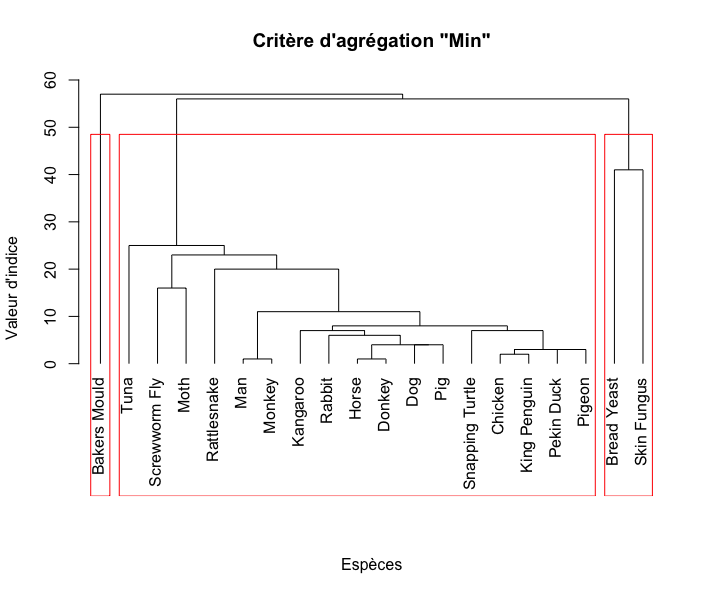
\includegraphics[width=1\linewidth]{img/2-1-mut-hierarchie-min}
		\caption{\scriptsize Critère agrégation Min}
		\label{fig:2-1-mut-hierarchie-min}
	\end{subfigure}%
	\begin{subfigure}[b]{0.4\linewidth}
		\centering
		\captionsetup{justification=centering}
		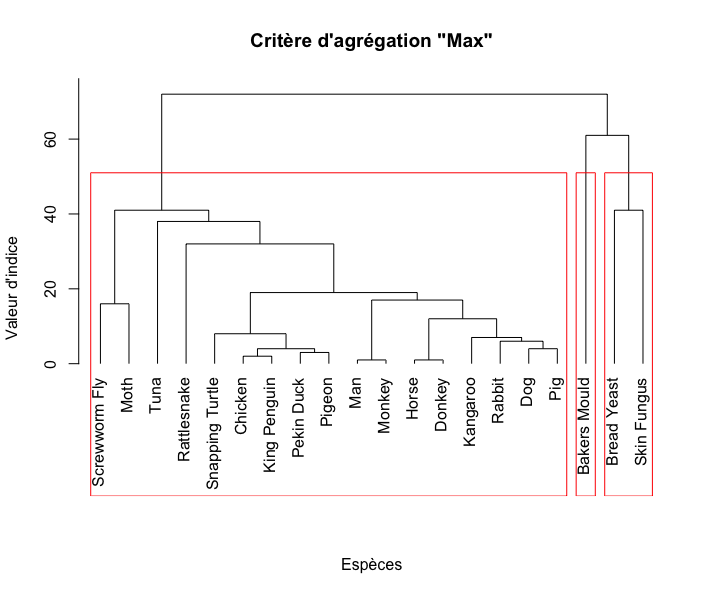
\includegraphics[width=1\linewidth]{img/2-1-mut-hierarchie-max}
		\caption{\scriptsize Critère agrégation Max}
		\label{fig:2-1-mut-hierarchie-max}
	\end{subfigure}%
	\caption{\small Classification avec les critères d'agrégation Min et Max}
	\label{fig:2-1-classification-mut-min-max}%
\end{figure}

\begin{figure}[H]
	\centering
	\captionsetup{justification=centering, margin=3cm}
	\begin{subfigure}[b]{0.4\linewidth}
		\centering
		\captionsetup{justification=centering}
		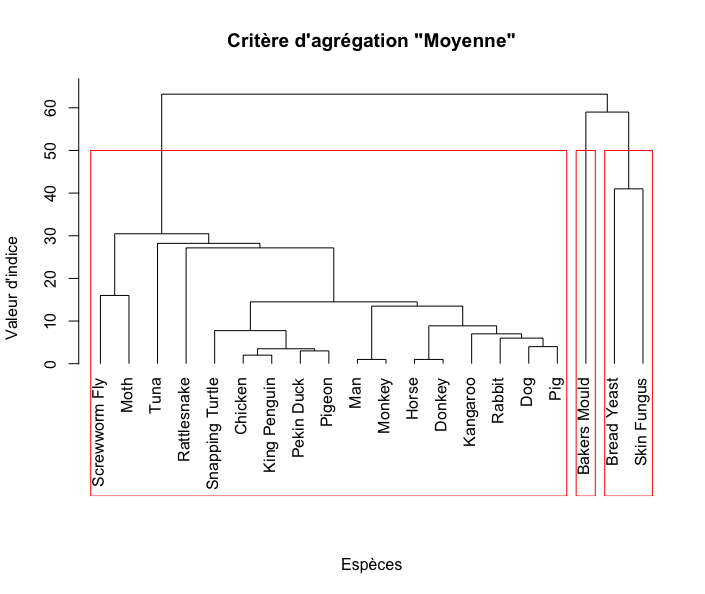
\includegraphics[width=1\linewidth]{img/2-1-mut-hierarchie-moy}
		\caption{\scriptsize Critère agrégation Moyenne}
		\label{fig:2-1-mut-hierarchie-moy}
	\end{subfigure}%
	\begin{subfigure}[b]{0.4\linewidth}
		\centering
		\captionsetup{justification=centering}
		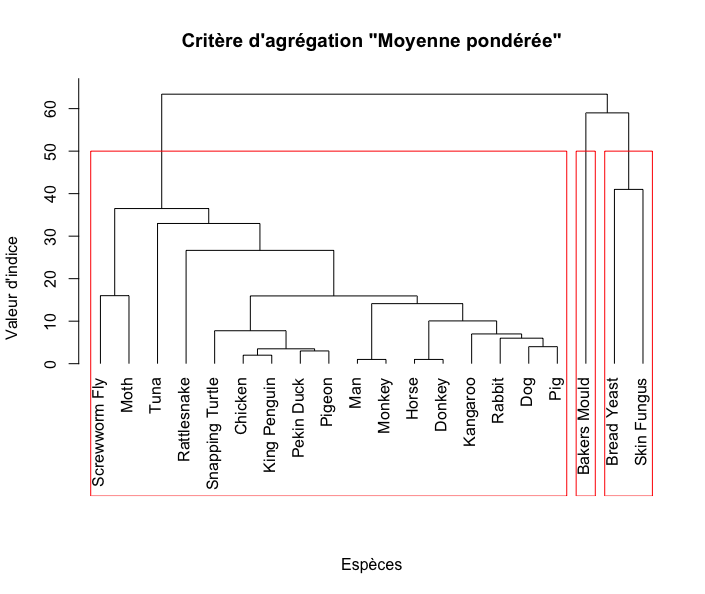
\includegraphics[width=1\linewidth]{img/2-1-mut-hierarchie-moy-ponderee}
		\caption{\scriptsize Critère agrégation Moyenne pondérée}
		\label{fig:2-1-mut-hierarchie-moy-ponderee}
	\end{subfigure}%
	\caption{\small Classification avec les critères d'agrégation Moyenne et Moyenne pondérée}
	\label{fig:2-1-classification-mut-moy}%
\end{figure}


\begin{figure}[H]
	\centering
	\captionsetup{justification=centering, margin=3cm}
	\begin{subfigure}[b]{0.4\linewidth}
		\centering
		\captionsetup{justification=centering}
		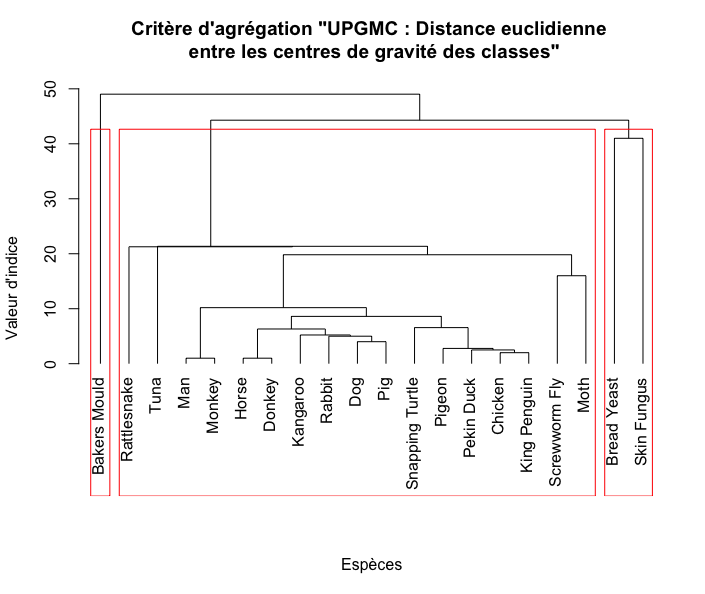
\includegraphics[width=1\linewidth]{img/2-1-mut-hierarchie-centroid}
		\caption{\scriptsize Critère agrégation distance inter-classe}
		\label{fig:2-1-mut-hierarchie-centroid}
	\end{subfigure}%
	\begin{subfigure}[b]{0.4\linewidth}
		\centering
		\captionsetup{justification=centering}
		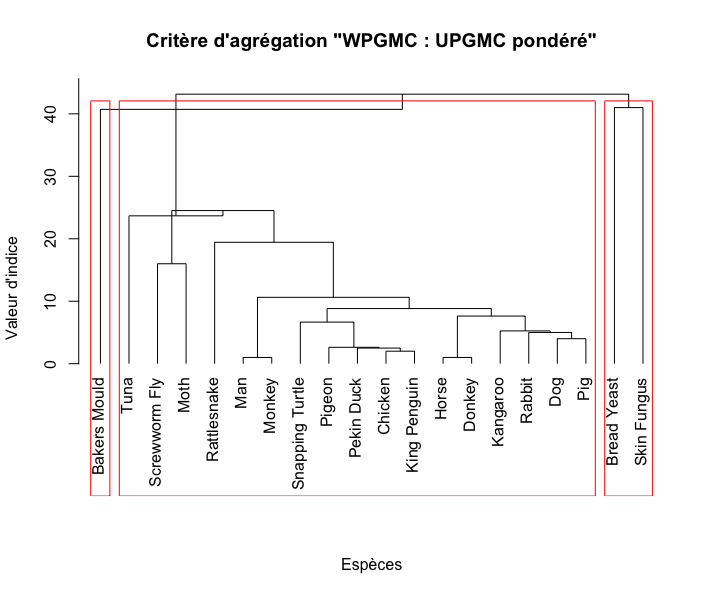
\includegraphics[width=1\linewidth]{img/2-1-mut-hierarchie-centroid-ponderee}
		\caption{\scriptsize Critère agrégation distance inter-classe pondérée}
		\label{fig:2-1-mut-hierarchie-centroid-ponderee}
	\end{subfigure}%
	\caption{\small Classification avec les critères d'agrégation de distance inter-classe (distance entre centres de gravité des classes)}
	\label{fig:2-1-classification-mut-centroid}%
\end{figure}


\begin{figure}[H]
	\centering
	\captionsetup{justification=centering, margin=3cm}
	\begin{subfigure}[b]{0.4\linewidth}
		\centering
		\captionsetup{justification=centering}
		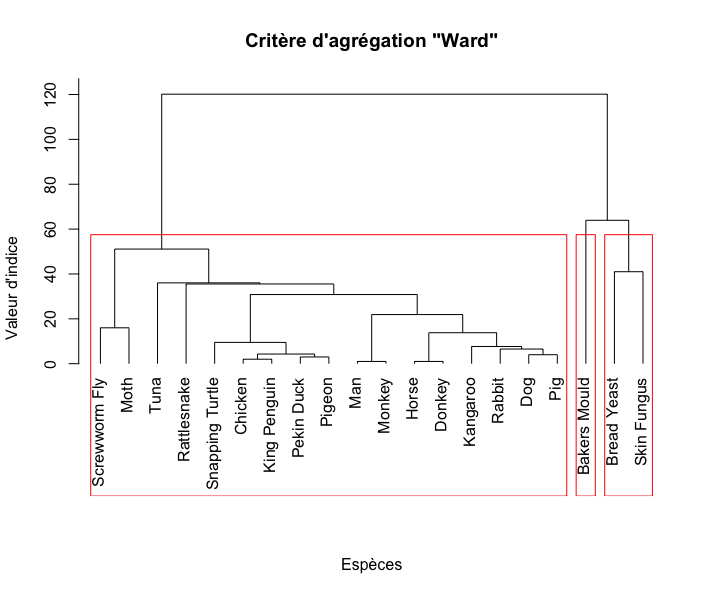
\includegraphics[width=1\linewidth]{img/2-1-mut-hierarchie-ward}
		%\caption{\scriptsize Critère agrégation Ward}
		\label{fig:2-1-mut-hierarchie-ward}
	\end{subfigure}%
	\caption{\small Classification avec le critère d'agrégation de Ward}
	\label{fig:2-1-classification-mut-ward}%
\end{figure}



La première chose qu'on remarque est que, lorsqu'on divise en trois classes tel que nous le suggérait la représentation graphique des données après AFTD (cf. \autoref{subsection:1-3-1-mut-premier-plan-factoriel}), tous les critères d'agrégation donnent les mêmes classes. A savoir \textit{\{Bakers Mould\}}, \textit{\{Bread Yeast, Skin Fungus\}}, et le reste dans la dernière classe.

Il est aussi intéressant de remarque que deux des critères d'agrégation ne sont pas monotones (cf. \autoref{fig:2-1-mut-hierarchie-centroid} et \autoref{fig:2-1-mut-hierarchie-centroid-ponderee}). On voit en effet que l'indice n'est pas décroissant.



\section{Classification hiérarchique sur les données Iris}



\subsection{Classification hiérarchique ascendante}

\begin{figure}[H]
	\centering
	\captionsetup{justification=centering, margin=3cm}
	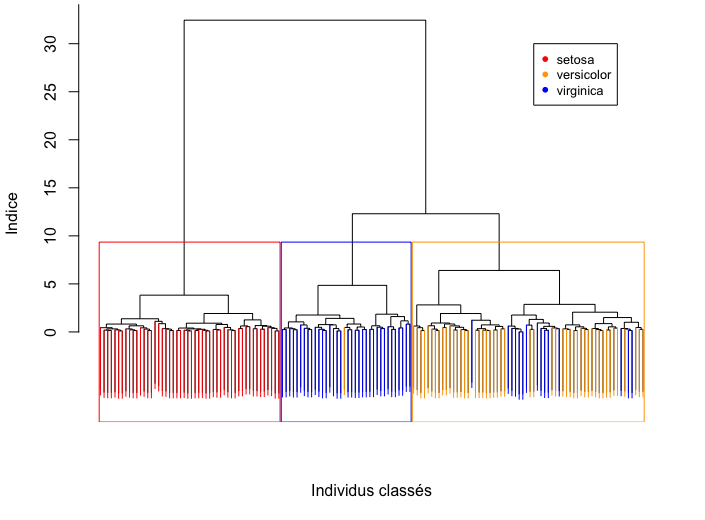
\includegraphics[width=.6\linewidth]{img/2-2-1-iris-class-hierarchique-asc}
	\caption{Iris : classification hiérarchique ascendante}
	\label{2-2-1-iris-class-hierarchique-asc}%
\end{figure}

La classification identifie très bien les individus de l'espèce \textit{setosa}. Par contre, elle tend à confondre certains individus des espèces \textit{versicolor} et \textit{virginica}. Compte tenu de la représentation graphique obtenue après ACP (cf. \autoref{fig:1-iris-acp-premier-plan-factoriel-discr-species}), ce n'est pas étonnant, ces deux espèces étant très proches sur le graphe, contrairement à \textit{setosa} qui est bien distincte.


\subsection{Classification hiérarchique descendante}

\begin{figure}[H]
	\centering
	\captionsetup{justification=centering, margin=3cm}
	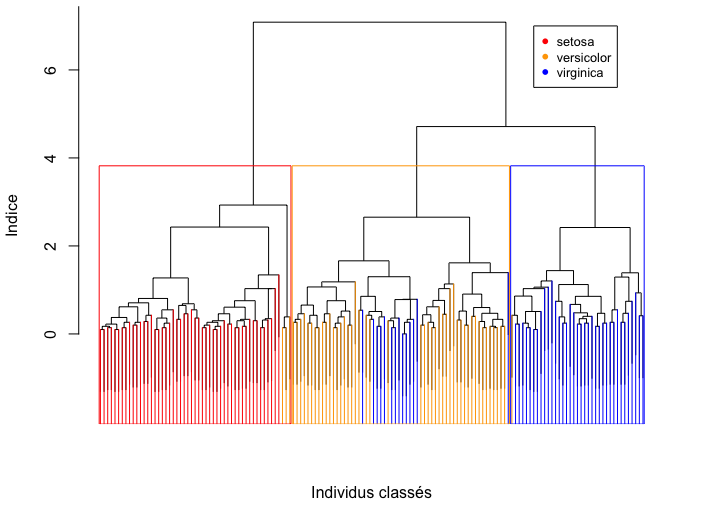
\includegraphics[width=.6\linewidth]{img/2-2-1-iris-class-hierarchique-desc}
	\caption{Iris : classification hiérarchique descendante}
	\label{2-2-1-iris-class-hierarchique-desc}%
\end{figure}


La classification hiérarchique descendante confond elle aussi certains des individus des espèces \textit{versicolor} et \textit{virginica}.
Afin de savoir laquelle des deux méthodes reste la plus précise, nous utilisons l'indice de Rand corrigé. Le principe est de sélectionner l'ensemble des paires possibles d'individus au sein de chaque partition et comparer leur classement au classement initial qui est connu. La valeur de cet indice est comprise entre 0 et 1~: plus elle se rapproche de 1, plus la classification obtenue est proche de la classification initiale.\\

Valeurs obtenues~:
\begin{itemize}
	\item Classification ascendante~: 0.73
	\item Classification descendante~: 0.69
\end{itemize}

On en déduit que la classification ascendante est meilleure pour ce jeu de données, bien que de peu.




\chapter{Méthode des centres mobiles (K-Means)}



\section{Données Iris}


\subsection{Partition en $K \in {2,3,4}$}


\subsection{Étude de la stabilité du résultat}


\subsection{Détermination du nombre de classes optimal}


\subsection{Comparaison de la classification obtenue avec la classification initiale}






\section{Données Crabs}

\subsection{Classification en 2 classes}


\subsection{Classification en 4 classes}

















\section{Données Mutations}



\subsection{Classification en 3 classes}


\subsection{Étude de la stabilité du résultat}

\end{document}